\section{Basic Definitions}
\label{sec:A.1}

This appendix contains an informal review of Markov chains. The aim is to describe briefly and
intuitively some of the main concepts and ideas that are important to understand Markov chain
Monte Carlo algorithms.

\begin{definition}[Markov Chain]
\label{def:A.1}
A collection $\mathbb{X} = \{X_n,\, n = 0, 1, 2, \ldots\}$ of random variables taking values in a
state space $E$ is called a Markov chain if
\[
  \Prob(X_{n+1} \in A_{n+1} \mid X_n \in A_n, \ldots, X_0 \in A_0)
  = \Prob(X_{n+1} \in A_{n+1} \mid X_n \in A_n)
\]
for all $n \geq 0$, and all measurable $A_{n+1}, A_n, \ldots, A_0 \subset E$.
\end{definition}

The index $n$ is often interpreted as time, and the Markov property then states that the future
(time $n+1$) is independent of the past (times $\leq n-1$) given the present (time $n$).

\begin{definition}[Time Homogeneous Markov Chain; Markov Kernel]
\label{def:A.2}
A Markov chain $\mathbb{X}$ is called time homogeneous if its transition probabilities
\[
  P(x, A) = \Prob(X_{n+1} \in A \mid X_n = x)
\]
do not depend on $n$. $P(x, A)$ is called the transition kernel or Markov kernel of $\mathbb{X}$.
\end{definition}

Here and below, the expression $\Prob(X_{n+1} \in A \mid X_n = x)$ is only formal if $\Prob(X_n = x) = 0$,
but it can be made rigorous using regular conditional probability.  From now on, all Markov
chains that we consider will be time homogeneous.  We will work mainly with transition kernels
that are absolutely continuous with respect to the Lebesgue measure or with respect to the counting
measure (an exception will be the Metropolis Hastings kernel studied in Chapter~4).  This
means that, for every $x$, there is an associated p.d.f.\ (or p.m.f.\ for the discrete case)
$p(x, z)$ such that
\[
  P(x, A) = \int_A p(x, z)\, dz.
\]
With slight abuse of terminology, we will often call $p(x, z)$ a Markov kernel.

\begin{example}[Weather Markov Chain]
\label{ex:A.3}
Suppose $X_n \equiv \text{weather at day } n =
\begin{cases}
  0 & \text{if sunny,} \\
  1 & \text{if cloudy,} \\
  2 & \text{if rainy.}
\end{cases}$

The state space is $E = \{0, 1, 2\}$.  We may specify (time homogeneous) transition probabilities
graphically as follows:

\begin{center}
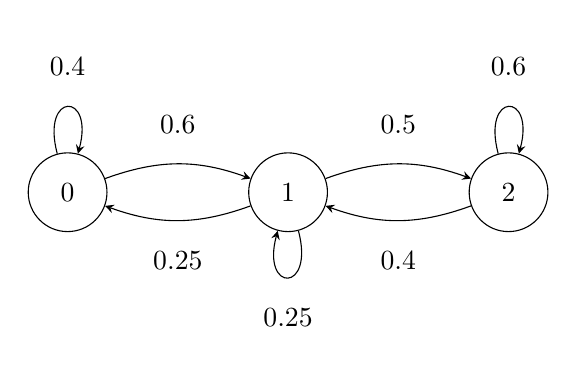
\begin{tikzpicture}[
    node distance=2.8cm,
    every node/.style={circle, draw, minimum size=1cm},
    >=stealth
  ]
  \node (S) {$0$};
  \node (C) [right of=S] {$1$};
  \node (R) [right of=C] {$2$};
  \draw[->] (S) to[loop above] node[draw=none,above] {$0.4$} (S);
  \draw[->] (S) to[bend left=20] node[draw=none,above] {$0.6$} (C);
  \draw[->] (C) to[bend left=20] node[draw=none,above] {$0.5$} (R);
  \draw[->] (C) to[loop below] node[draw=none,below] {$0.25$} (C);
  \draw[->] (C) to[bend left=20] node[draw=none,below] {$0.25$} (S);
  \draw[->] (R) to[loop above] node[draw=none,above] {$0.6$} (R);
  \draw[->] (R) to[bend left=20] node[draw=none,below] {$0.4$} (C);
\end{tikzpicture}
\end{center}
\end{example}

\begin{definition}[$n$-th Step Transition Densities]
\label{def:A.4}
The $n$-th step transition probability densities $p^n(x, z)$ are defined by
\[
  \Prob(X_n \in A \mid X_0 = x) = P^n(x, A) = \int_A p^n(x, z)\, dz.
\]
\end{definition}

If the state space is finite, say $E = \{0, 1, \ldots, s\}$ for some integer $s$, then we can collect
the transition probabilities in the \emph{transition matrix}
\[
  P = [p_{ij}]_{i,j \in E},
\]
where $p_{ij} = \Prob(X_{n+1} = j \mid X_n = i)$ for $(i, j) \in E \times E$.  It holds that
\[
  p^n(i, j) = (P^n)_{ij}.
\]

\begin{lemma}
\label{lem:A.5}
If $X_0 \sim \pi_0$ and $\mathbb{X}$ has $n$-th step transition probability densities $p^n(x, z)$,
then the p.d.f.\ of $X_n$ is given by
\[
  \pi_n(x) = \int_E \pi_0(z)\, p^n(z, x)\, dz.
\]
If the state space $E$ is finite, then $\pi_n$ is the probability vector given by $\pi_n = \pi_0 P^n$.
\end{lemma}

\begin{example}[Weather Markov Chain: 2-Step Probabilities]
\label{ex:A.6}
The transition matrix of the weather chain is given by
\[
  P = \begin{bmatrix} 0.4 & 0.6 & 0 \\ 0.25 & 0.25 & 0.5 \\ 0 & 0.4 & 0.6 \end{bmatrix}.
\]
Suppose day~0 is sunny.  Then,
\[
  \pi_0 = \begin{bmatrix} 1 & 0 & 0 \end{bmatrix}.
\]
The distribution of the weather on day~2 is
\[
  \pi_2 = \pi_0 P^2 = \begin{bmatrix} 1 & 0 & 0 \end{bmatrix} P^2
         = \begin{bmatrix} 0.31 & 0.39 & 0.3 \end{bmatrix}.
\]
So if day~0 is sunny, then day~2 has a $0.31$ probability of being sunny.
\end{example}
